\documentclass[10pt,a4paper]{beamer}
\hypersetup{pdfstartview={Fit}}
\usetheme{Berkeley}
\usecolortheme{sidebartab}
\usepackage{color}
\usepackage{graphicx}
\usepackage{movie15,media9}
\setbeamertemplate{caption}[numbered]

\begin{document}
	\setbeamertemplate{sidebar left}{}
	\title{Progress Presentation-II}
	\subtitle{e-Yantra Summer Internship-2018 \\ $ $\textbf{A System for Solving Jigsaw Puzzle using Multiple Robots}$ $}
	\author{$ $Aniket Anantraj Navlur$ $\\$ $Ashis kumar Maharana$ $\\$ $Kiran S Patil$ $\\ \vspace{1em}
	Mentors: \\$ $Abhinav Sarkar, Kalind Karia$ $}
	\institute{IIT Bombay}
	\date{\today}
	%\addtobeamertemplate{sidebar left}{}{\includegraphics[scale = 0.3]{logowithtext.png}}
	\frame{\titlepage}

\setbeamertemplate{sidebar left}[sidebar theme]
\section{Overview of Project}
\begin{frame}{Overview of Project}
	
	\begin{itemize}
		\item \textcolor{blue}{Project Name:} A System for Solving Jigsaw Puzzle using Multiple Robots
		\item \textcolor{blue}{Objective:}
		\begin{itemize}
			\item To develop an autonomous system that can solve any Jigsaw Puzzle given its image using multiple robots 
		\end{itemize}
		\item \textcolor{blue}{Deliverables:}
		\begin{enumerate}
			\item Go-to-Goal controller for robot in a given frame
			\item Autonomous solving of any Jigsaw Puzzle given just its image
			\item Proper documentation and report on solution of the system
		\end{enumerate}
	\end{itemize}
\end{frame}

\section{Overview of Task}
\begin{frame}{Overview of Task}
	\begin{tabular}{| c | p{17.8 em} | c |}\hline
		\textbf{Task No.} & \hspace{7em}\textbf{Task} & \textbf{Status} \\\hline
		1 &\small{ Python, OpenCV, Firebird V Intro,\hspace{5 em}XBee Communication} & Done \\\hline
		2 &\small{ Pose and orientation calculation of 2 Firebird robots using color/Aruco markers }& Done\\\hline
		3 &\small{ Programming the Go-To-Goal Controller for single Firebird V robot. Tuning the PID\hspace{3 em} values to perfection }& Done\\\hline
		4 &\small{ Implementing path planning with Firebird V where obstacles have been placed in arena }& Done\\\hline
		5 &\small{ Detection of jigsaw puzzle blocks using\hspace{3 em}Template Matching} & Done\\\hline
		6 &\small{ Pick and place of blocks - gripper mechanism building }& Ongoing\\\hline
		7 &\small{ Implementing the entire solution for a given\hspace{3 em}jigsaw puzzle }& Ongoing\\\hline
		8 &\small{ Documentation and reporting results }& Pending\\\hline
	\end{tabular}
\end{frame}

\section{Task Accomplished}
\begin{frame}{Task Accomplished}
\begin{itemize}
\color{blue}
\item Template matching
\begin{itemize}
\color{olive}
\item without rotation
\item with rotation
\begin{columns}
\column{0.5\framewidth}
\begin{figure}
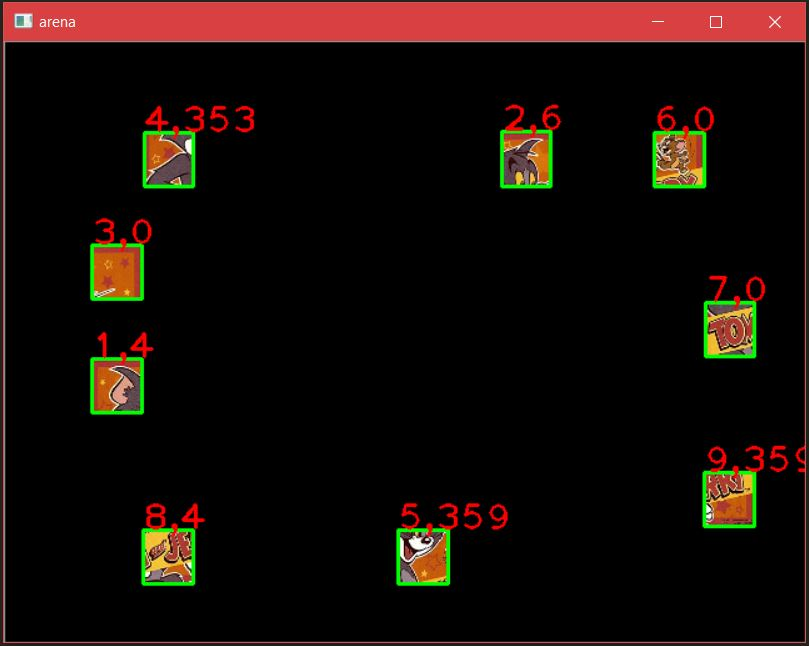
\includegraphics[height=0.35\textheight]{template.jpg}\caption{Puzzle block identified with orientation}
\end{figure}
\column{0.5\framewidth}
\begin{figure}
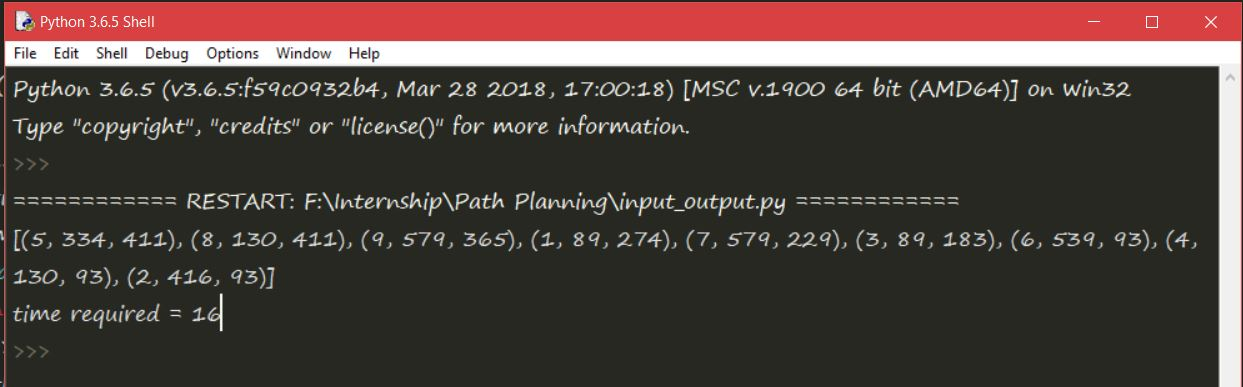
\includegraphics[height=0.3\textheight, width=1\textwidth]{templatem.jpg}\caption{Puzzle blocks with their center}
\end{figure}
\end{columns}
\end{itemize}
\item Introduction to CAD software
\begin{itemize}
\color{olive}
\item Fusion360
\item OpenSCAD
\end{itemize}
\item Gripper Mechanism
\item Path Planning with collision avoidance between Robots
\end{itemize}
\end{frame}

\begin{frame}{First 3D design}
\begin{columns}
\column{0.5\framewidth}
\begin{figure}
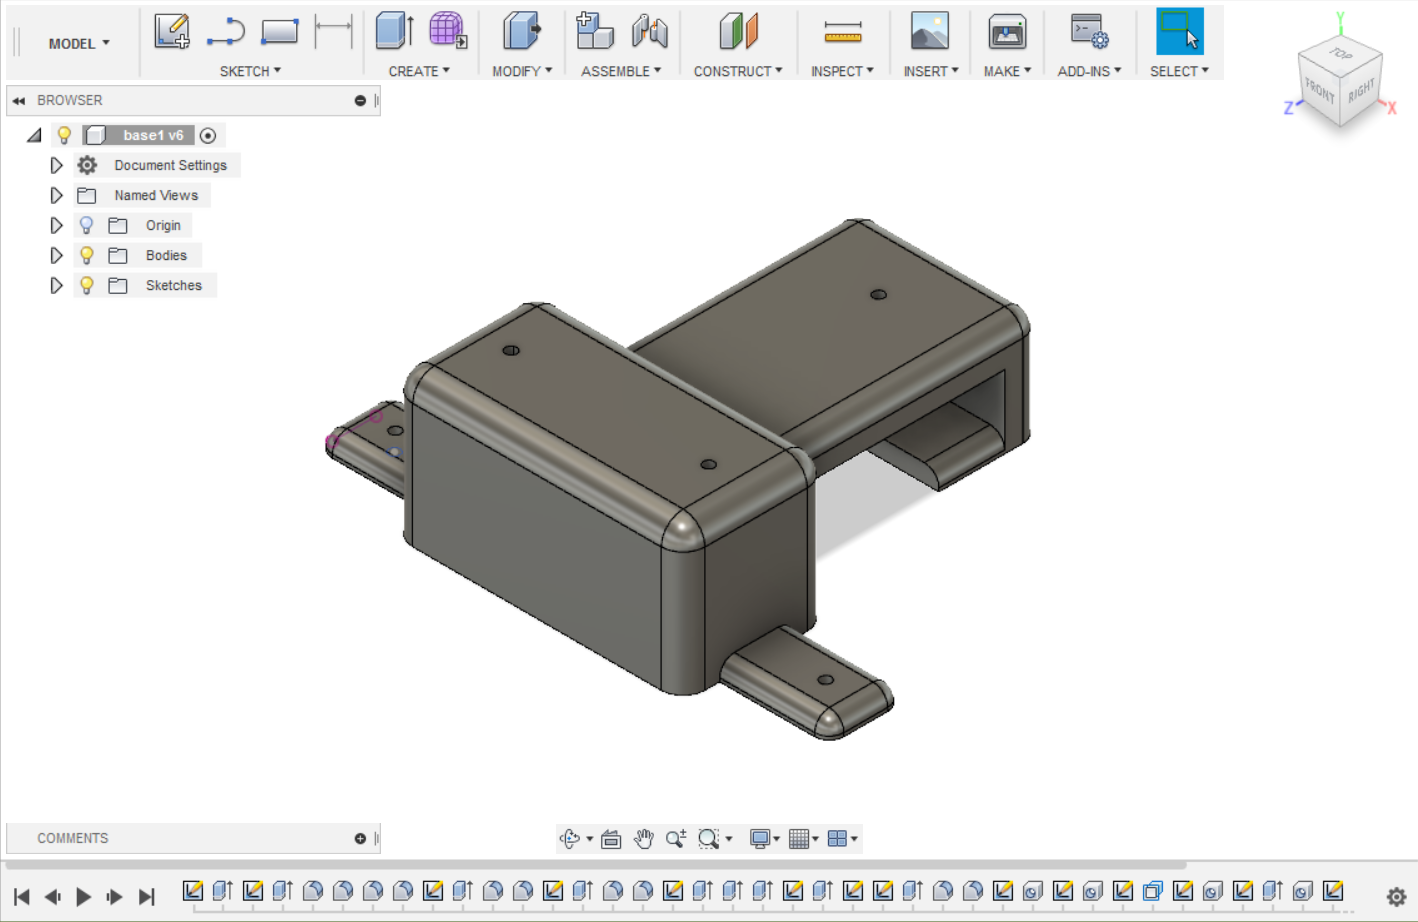
\includegraphics[height=0.2\textheight, width=0.35\framewidth]{Base.png}\caption{\small{Base}}
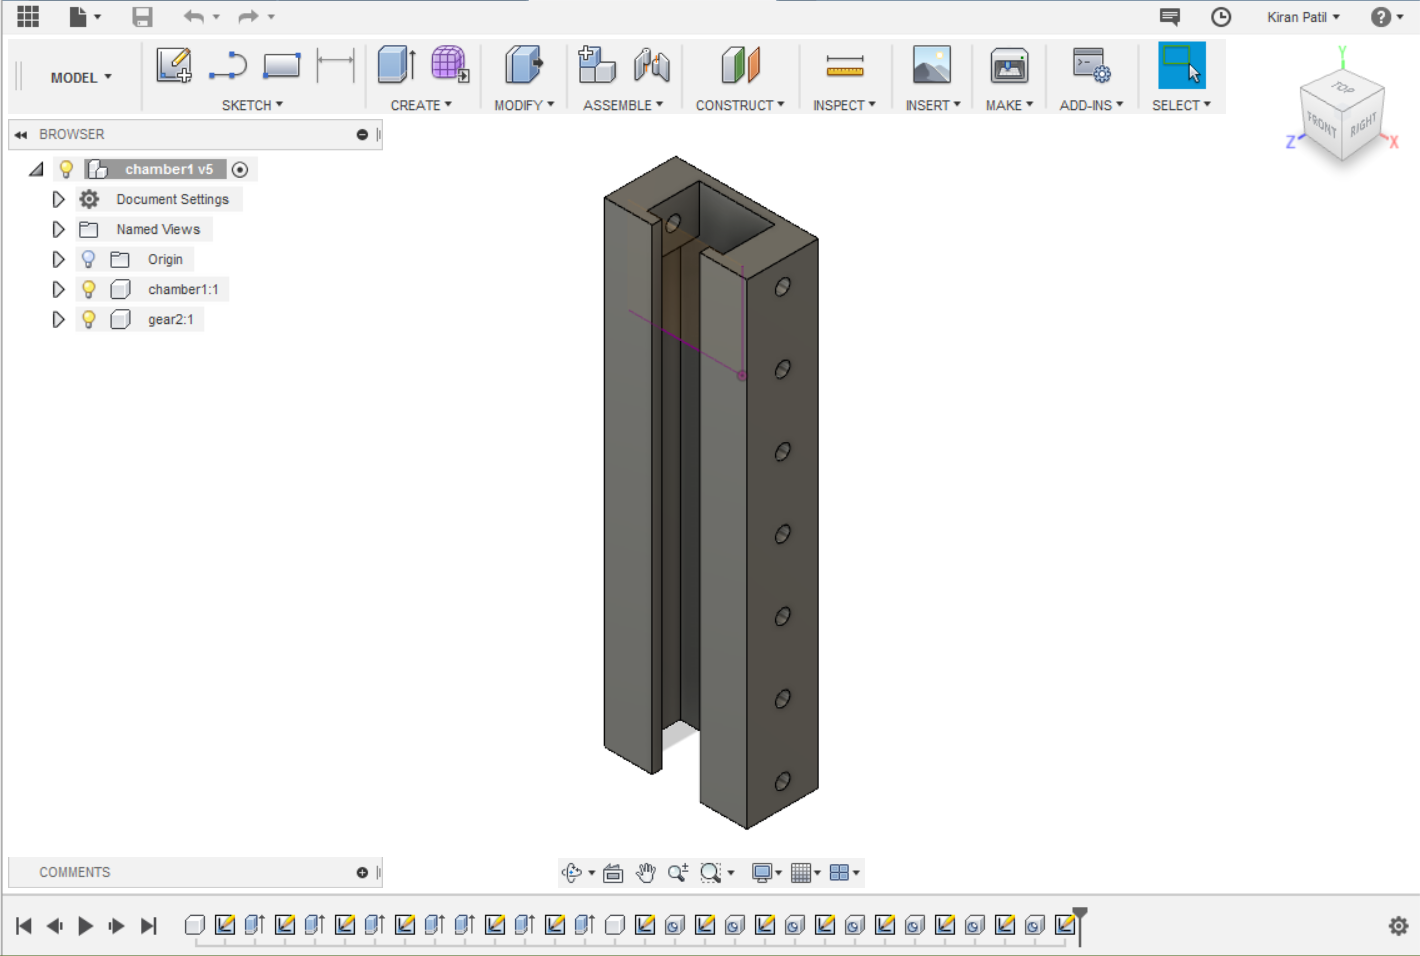
\includegraphics[height=0.2\textheight,  width=0.35\framewidth]{Chamber.png}\caption{\small{Chamber}}
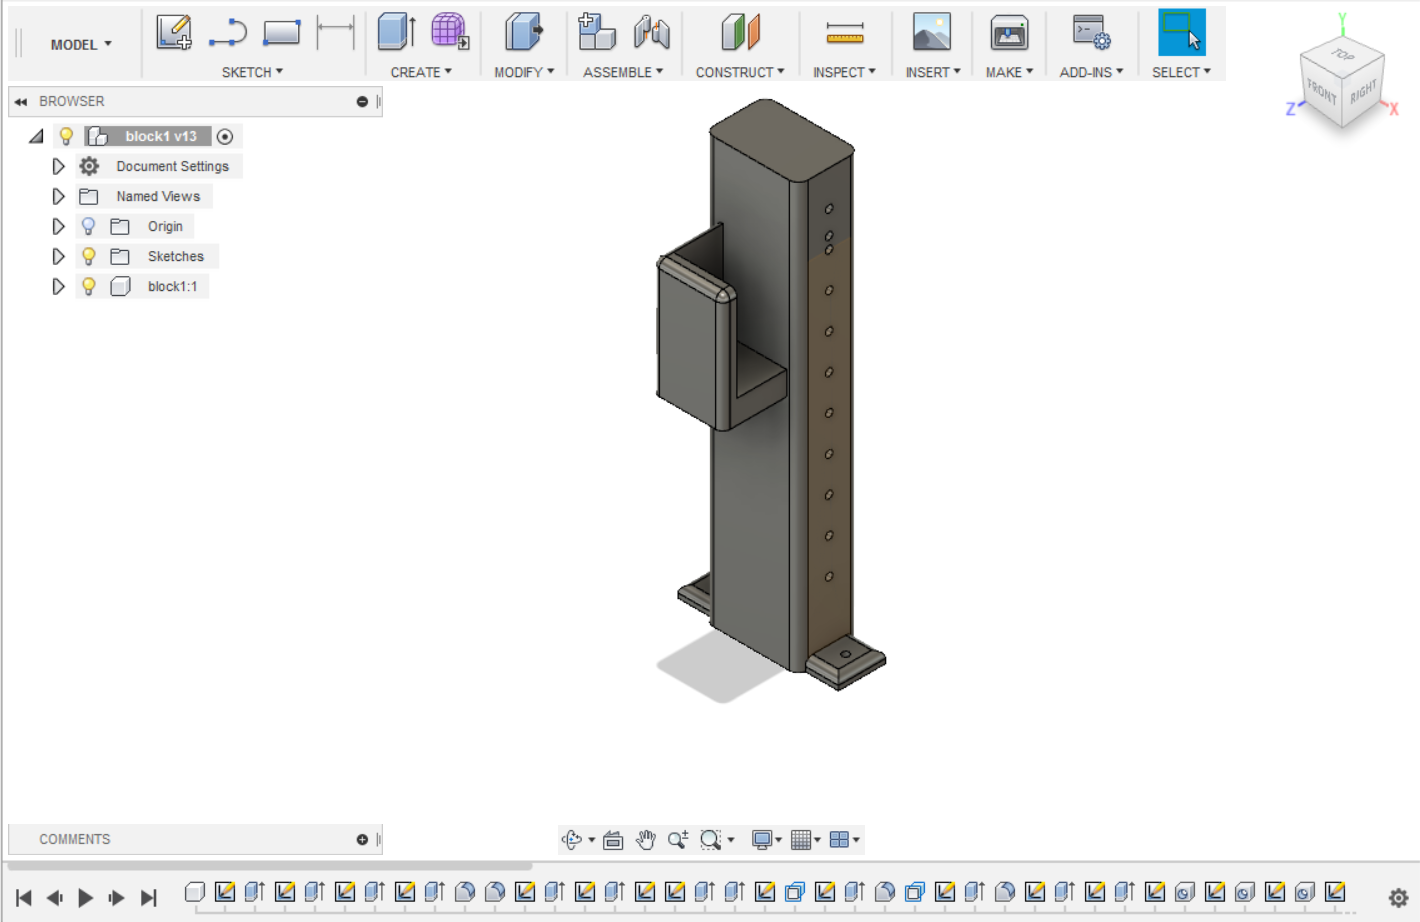
\includegraphics[height=0.2\textheight,  width=0.35\framewidth]{Column.png}\caption{\small{Column}}
\end{figure}
\column{0.5\framewidth}
\begin{figure}
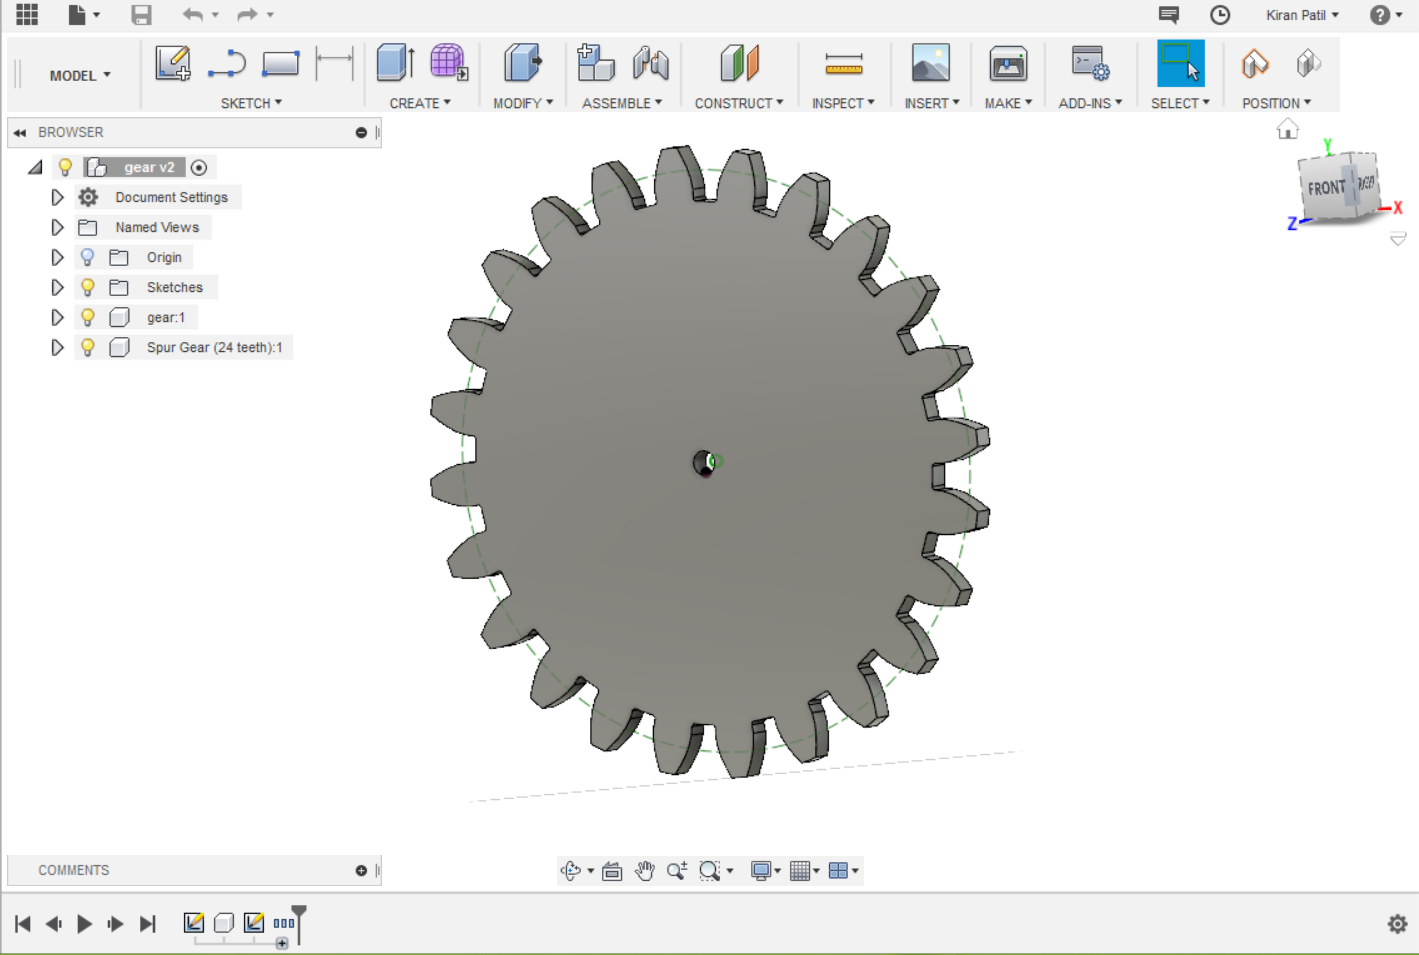
\includegraphics[height=0.3\textheight,  width=0.4\framewidth]{Gear.png}\caption{\small{Gear}}
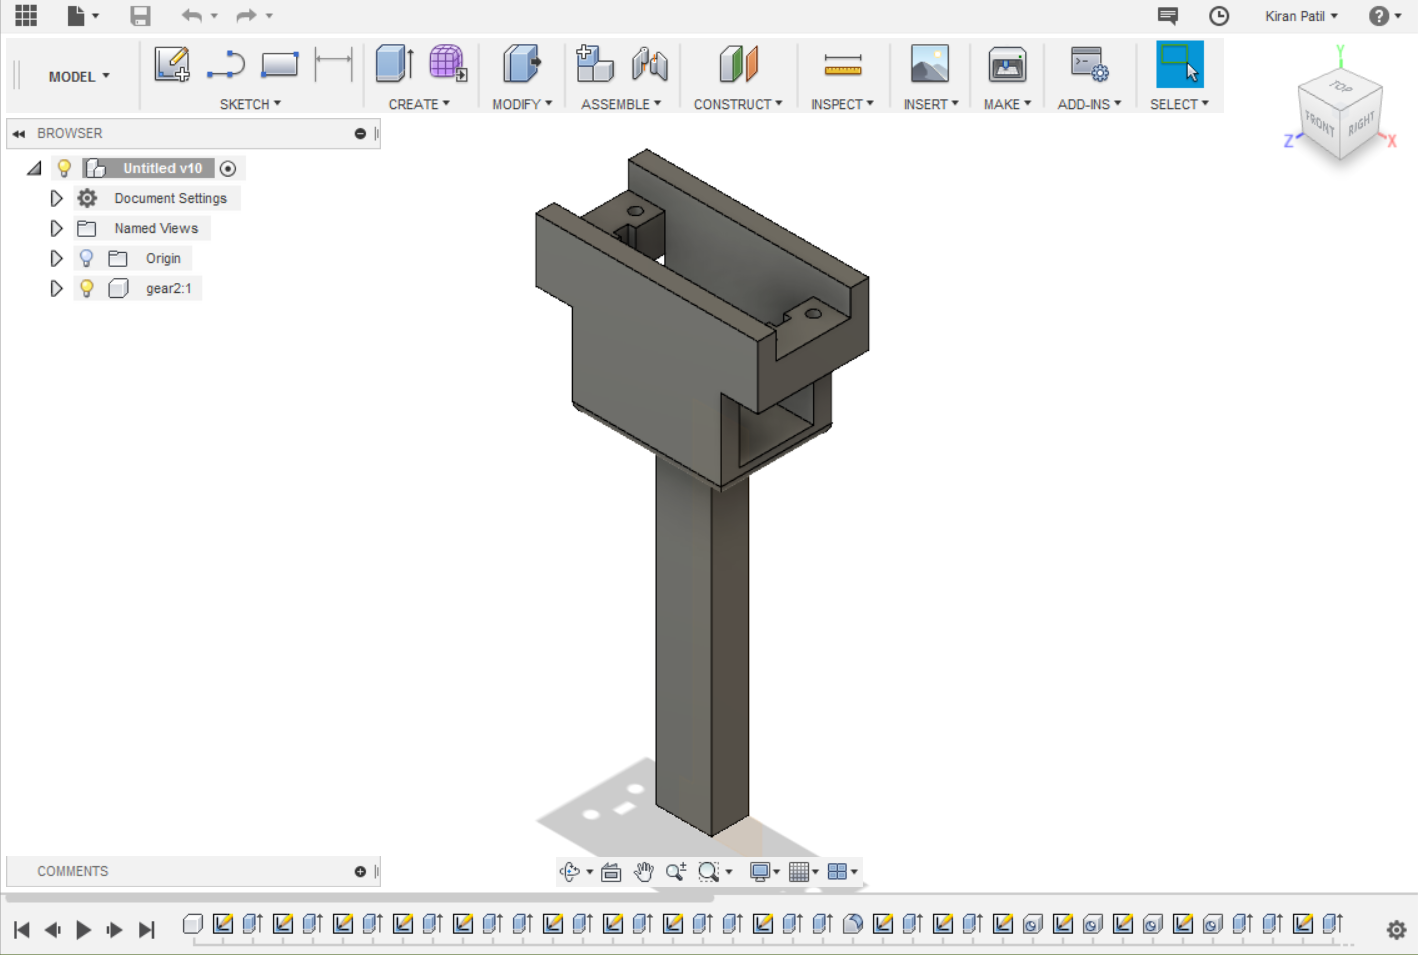
\includegraphics[height=0.3\textheight,  width=0.4\framewidth]{Rack_with_Servo_slot.png}\caption{\small{Rack with Servo slot}}
\end{figure}
\end{columns}
\end{frame}

\begin{frame}{Second 3D design}
\begin{columns}
\column{0.3\framewidth}
\begin{figure}
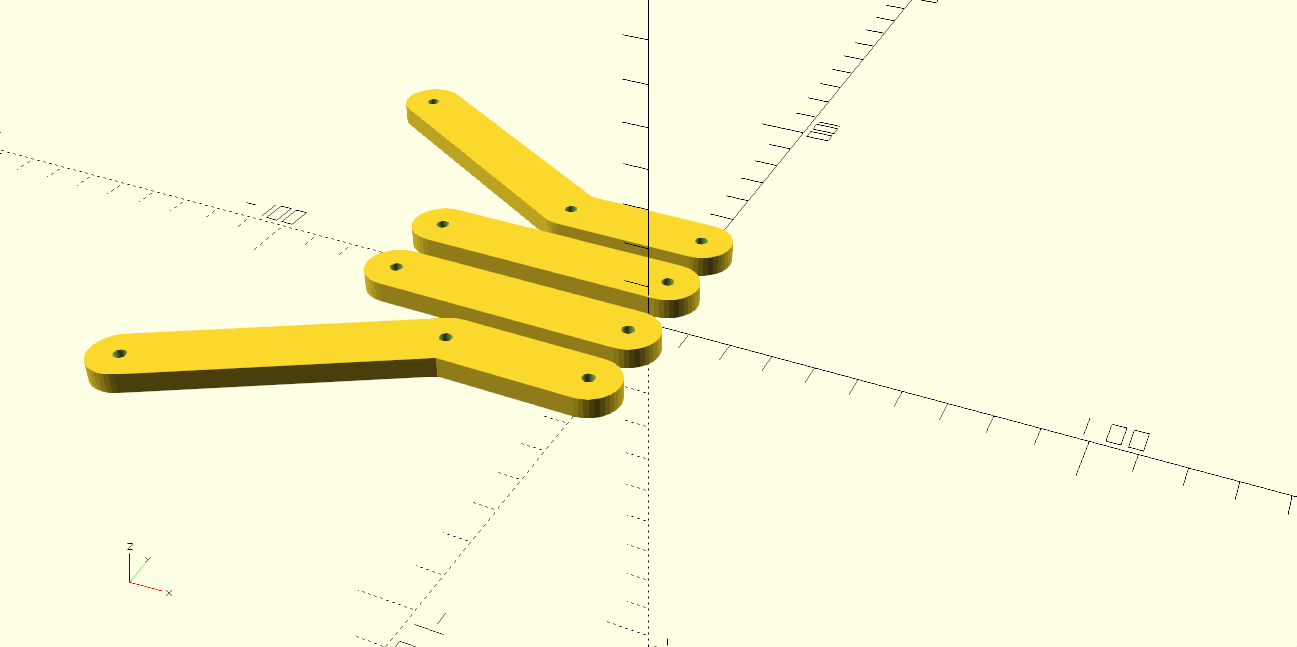
\includegraphics[scale=0.1]{Arms.png}\caption{\small{Arms}}
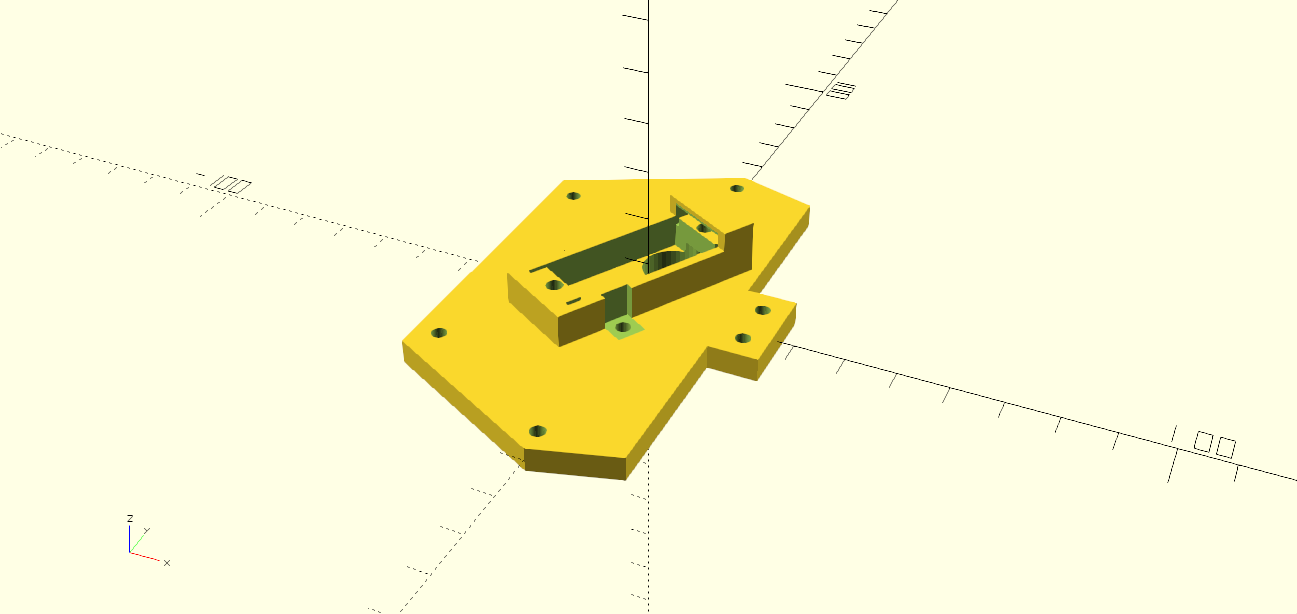
\includegraphics[scale=0.1]{BottomPlate.png}\caption{\small{BottomPlate}}
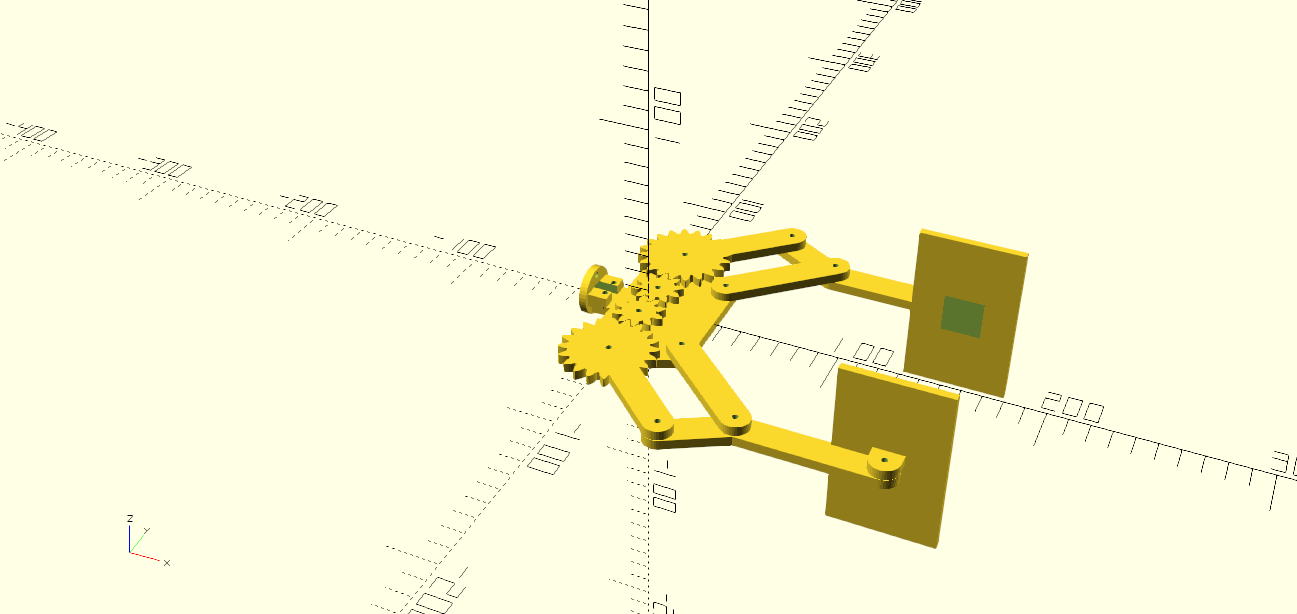
\includegraphics[scale=0.1]{Claw.png}\caption{\small{Claw}}
\end{figure}
\column{0.3\framewidth}
\begin{figure}
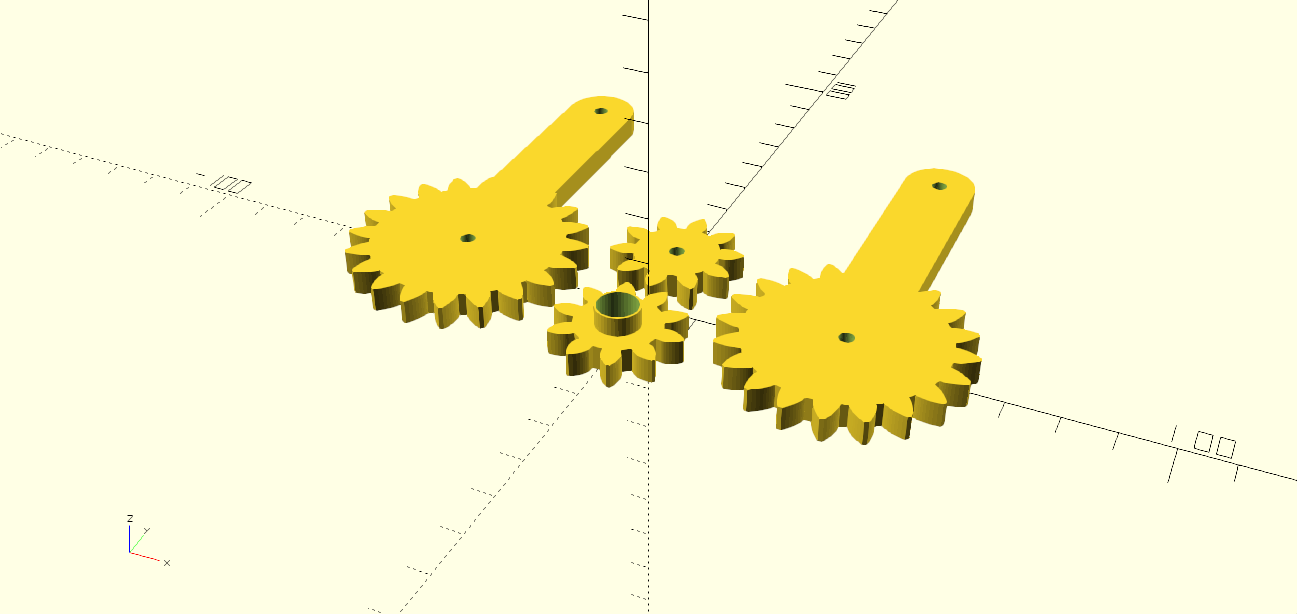
\includegraphics[scale=0.1]{Gears.png}\caption{\small{Gears}}
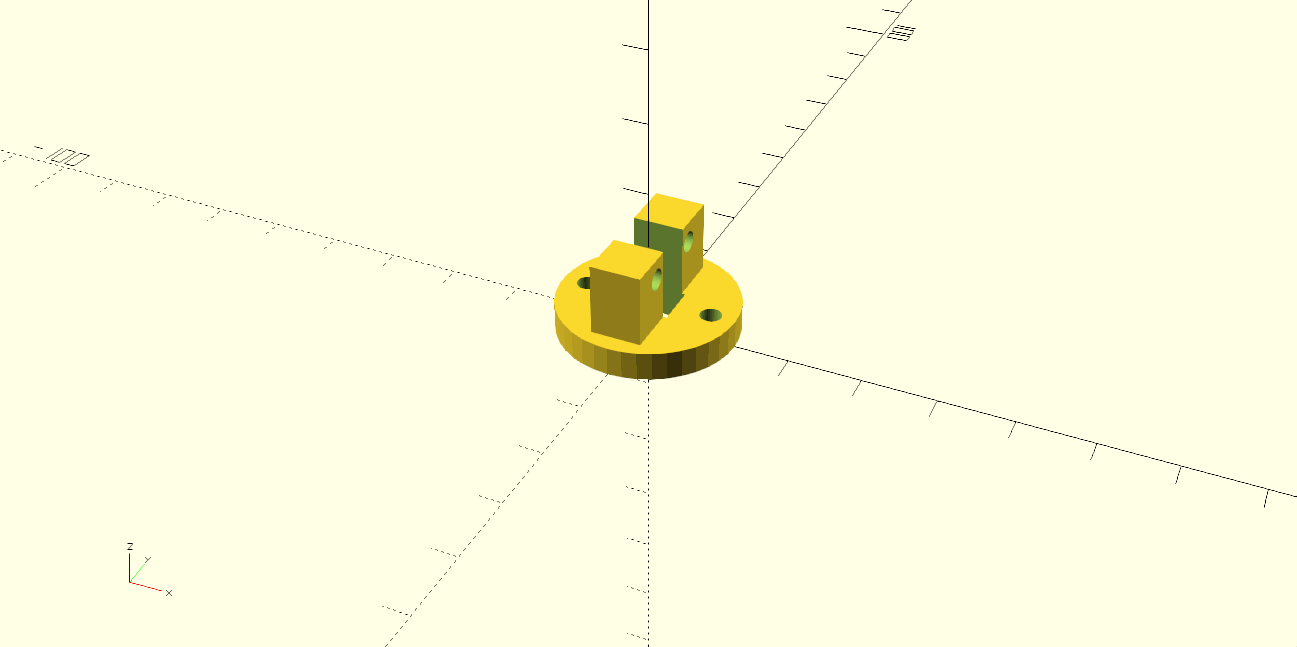
\includegraphics[scale=0.1]{ServoMount.png}\caption{\small{ServoMount}}
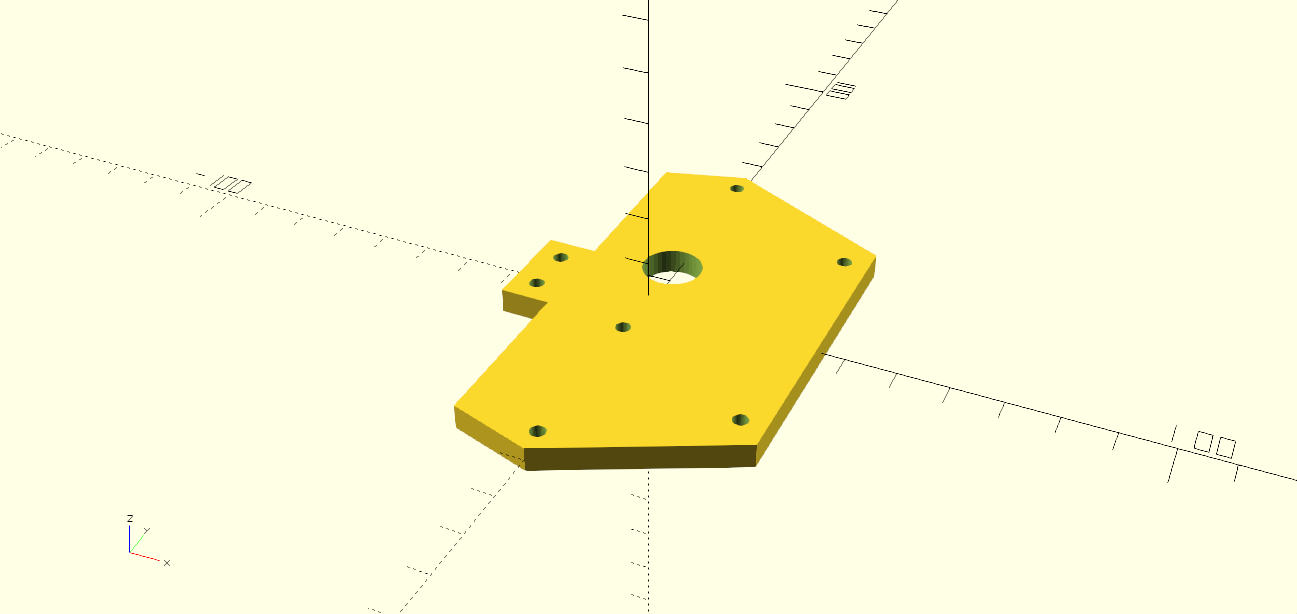
\includegraphics[scale=0.1]{TopPlate.png}\caption{\small{TopPlate}}
\end{figure}
\column{0.3\framewidth}
\begin{figure}
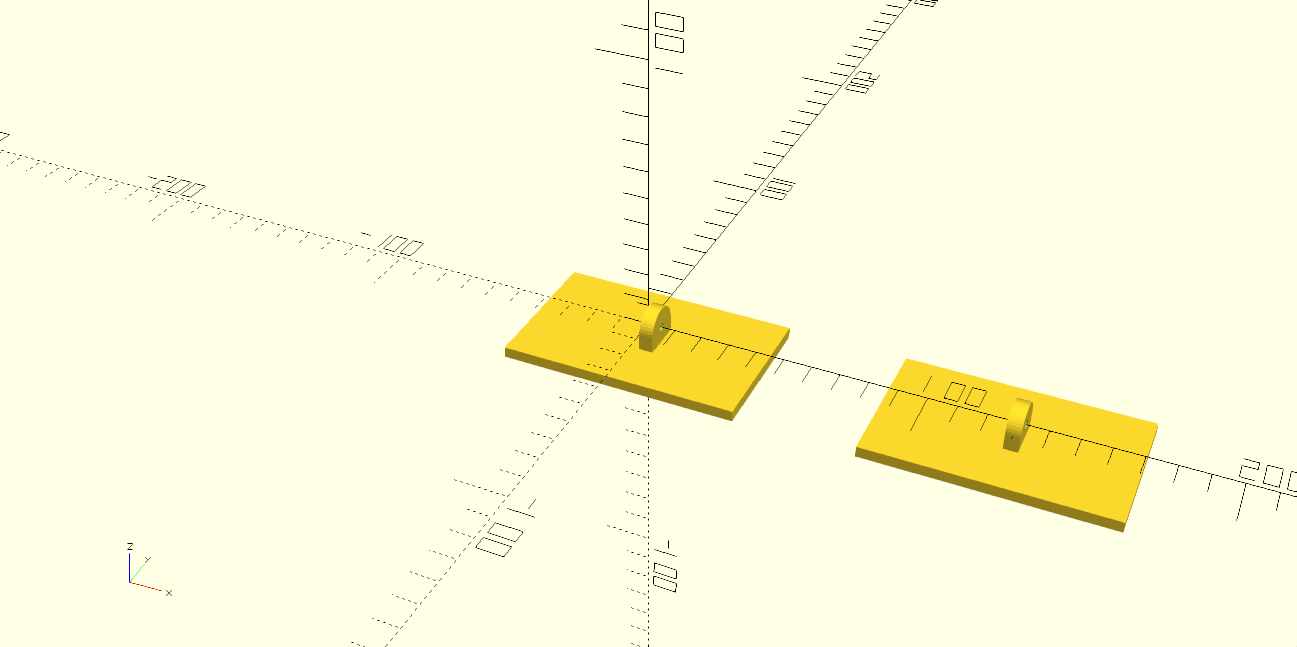
\includegraphics[scale=0.1]{GripperPlate.png}\caption{\small{GripperPlate}}
\end{figure}
\end{columns}
\end{frame}

\begin{frame}{Latest Design}
\begin{figure}
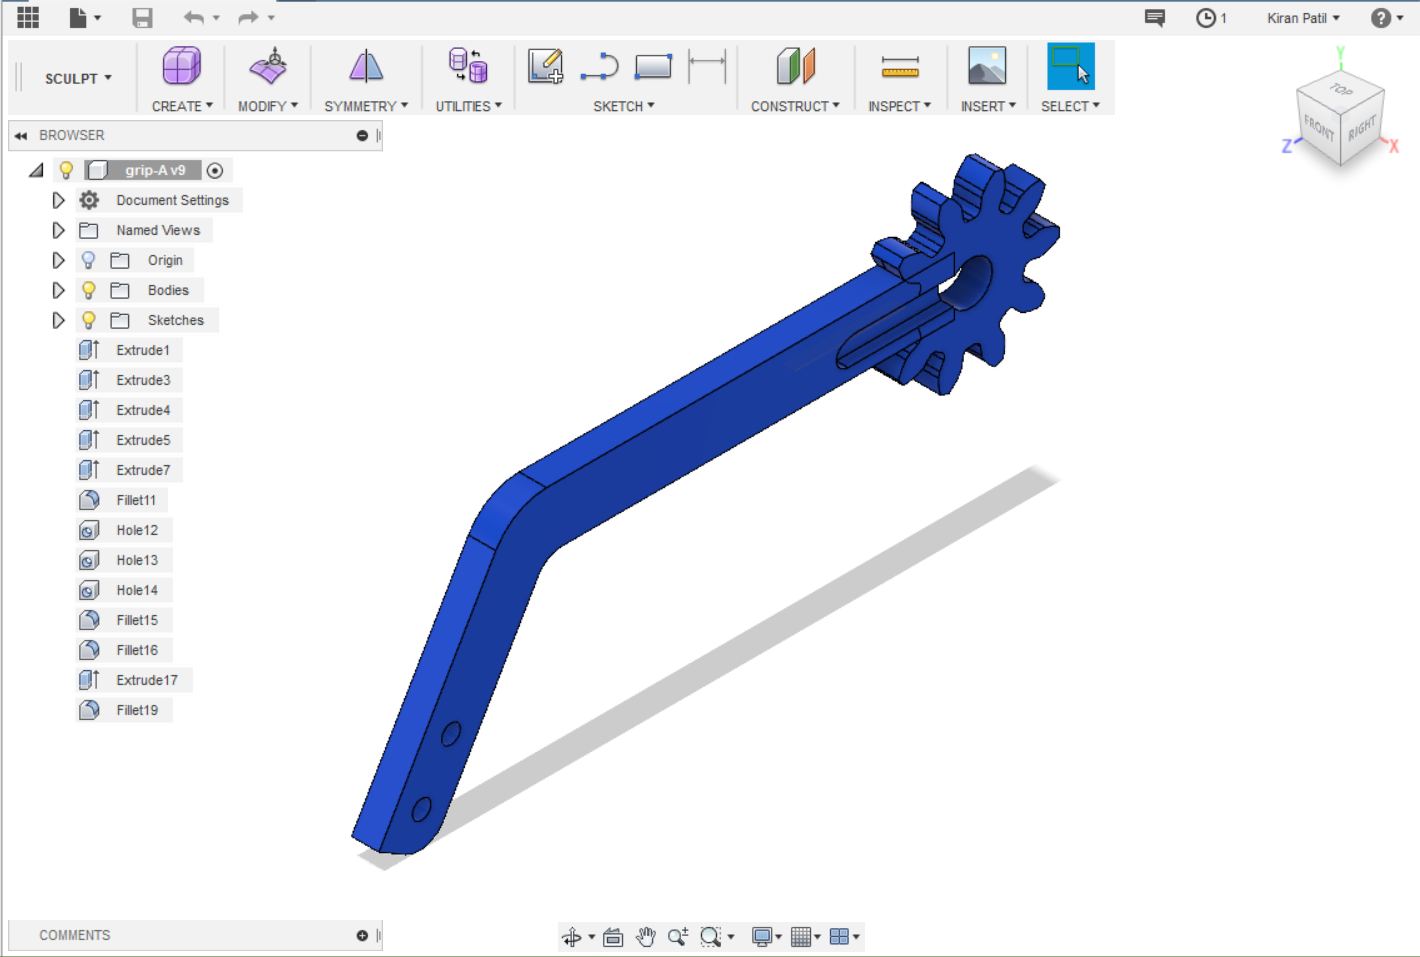
\includegraphics[height=0.2\textheight, width=0.3\textwidth]{gear1.png}\caption{Right Gear}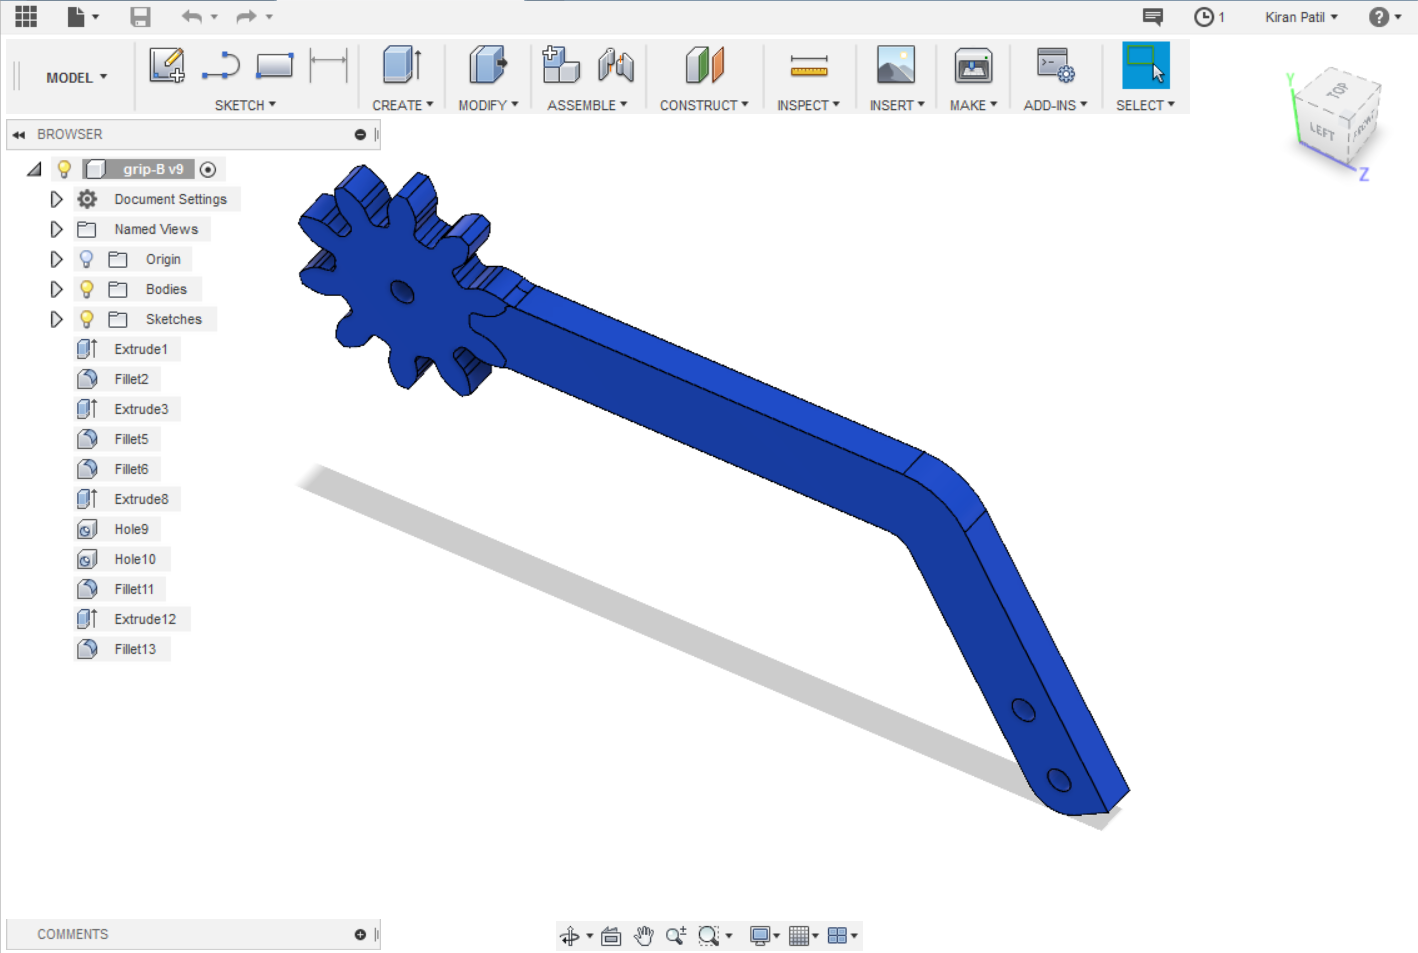
\includegraphics[height=0.2\textheight, width=0.3\textwidth]{gear2.png}\caption{Left Gear}
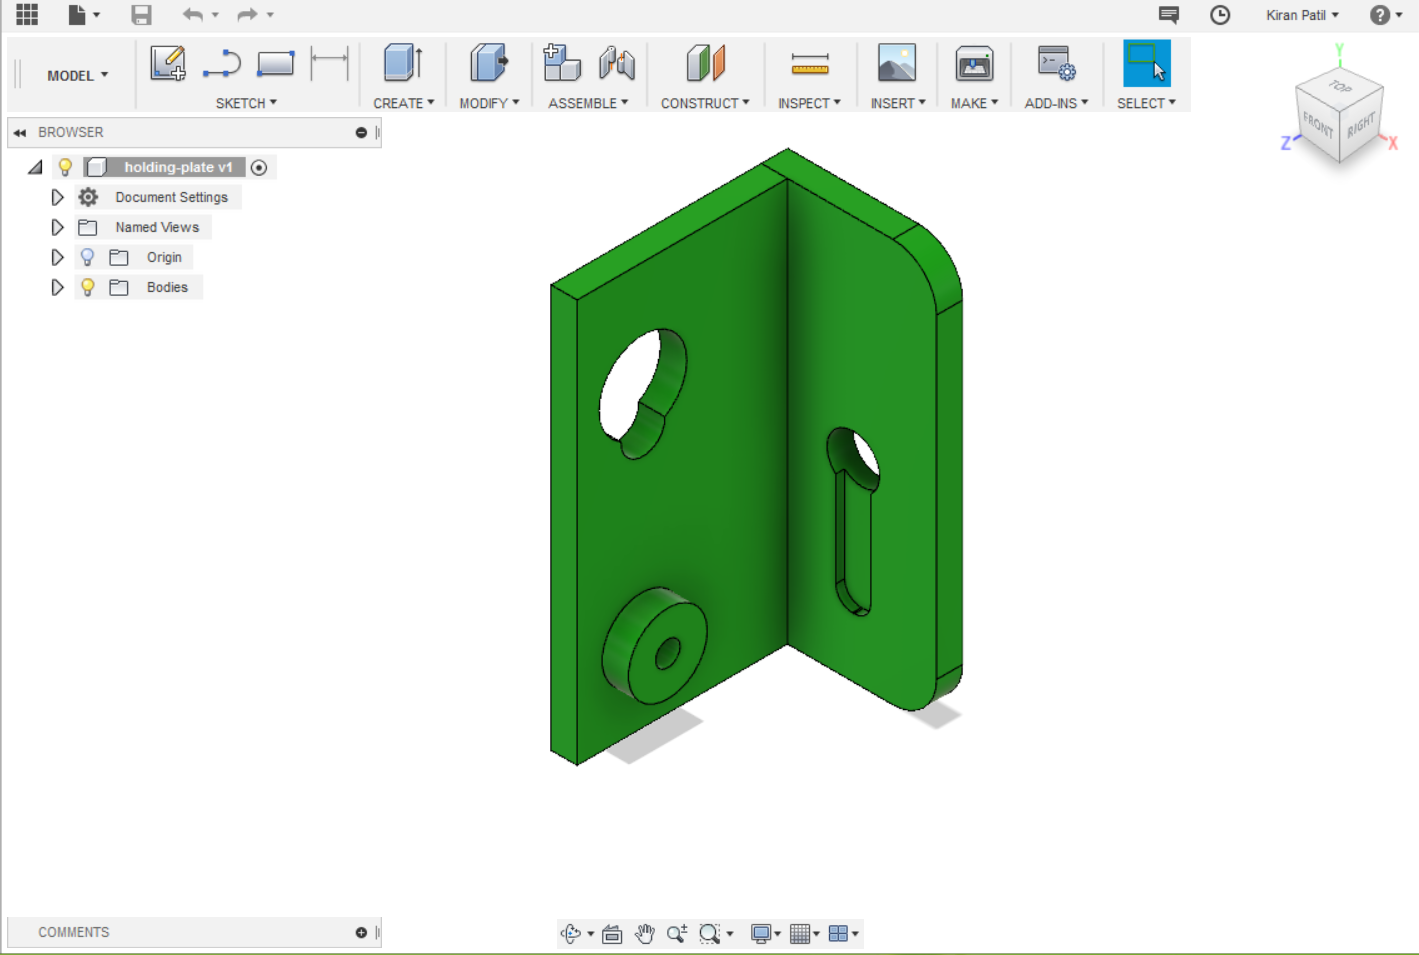
\includegraphics[height=0.2\textheight, width=0.3\textwidth]{plate.png}\caption{Servo Mount}
\end{figure}
\end{frame}
\section{Challenges Faced}
\begin{frame}{Challenges Faced}
	\begin{itemize}
	\color{red}
		\item Right gripper mechanism for the problem
		\item Block size and arm height(with 3 DOF) 
		\item The size of arena captured from the camera 
	\end{itemize}
\end{frame}

\section{Future Plans}
\begin{frame}{Future Plans}
	\begin{itemize}
	\color{violet}
		\item Implementation of whole of the solution to solve a puzzle
		\item Documentation
	\end{itemize}
\end{frame}


\section{Thank You}
\begin{frame}{Thank You}
	\centering\textcolor{violet} T\textcolor{purple}H\textcolor{blue}A\textcolor{green}N\textcolor{yellow}K \textcolor{orange}Y\textcolor{red}O\textcolor{gray}U !!!
\end{frame}
\end{document}
